% !TeX root = ../main.tex
% Add the above to each chapter to make compiling the PDF easier in some editors.

\chapter{Base Operating System: Axcan OS}\label{chap:os}

To enable the proposed breathable distributed real-time system — capable of dynamic task migration across heterogeneous embedded nodes — a shared, minimal, and portable operating system stack is essential. This stack must satisfy several core requirements: it must be lightweight enough to operate on constrained electronic control units (ECUs) and virtualized edge platforms; it must support real-time scheduling and task isolation across mixed-criticality workloads; and it must enable dynamic execution of precompiled applications without requiring platform-specific recompilation.

Existing operating systems typically fall short on one or more of these requirements. For example, lightweight RTOSes like FreeRTOS offer deterministic scheduling and minimal overhead, but lack support for dynamic task deployment and mixed-criticality scheduling. In contrast, general-purpose real-time operating systems like PREEMPT-RT Linux provide advanced scheduling and deployment capabilities but impose a significant memory and processing footprint unsuitable for many embedded platforms.

This chapter introduces Axcan OS, a custom operating system framework built as an extension to the FreeRTOS microkernel. Axcan OS forms the runtime foundation of the breathable system by enabling cross-platform, real-time execution of position-independent applications. It provides a unified abstraction for both physical ECUs and virtual nodes hosted in mobile edge computing (MEC) environments.

Axcan OS introduces several key features that address the challenges of distributed real-time execution in the proposed system:

\begin{itemize}
	\item Dynamic task deployment: a lightweight remote deployment manager receives and launches application binaries as decided by the system master node.
	
	\item Cross-platform execution: applications are compiled as position-independent ELF files that can be executed unmodified across compatible architectures. Furthermore,  system service abstraction provide consistent interfaces for system managed functions across heterogeneous nodes.
	
	\item Real-time capabilities: supports various scheduling policies, including preliminary mixed-criticality strategies, and provides global time synchronization using Precision Time Protocol (PTP).
\end{itemize}

The name of the operating system comes from the Nahuatl word \textit{axcan}, meaning “now” or “immediately,” reflecting the real-time responsiveness envisioned for the system.

The remainder of this chapter details the design, implementation, and integration of Axcan OS within the broader architecture, including its current limitations and future development directions.

\section{Architecture}
The architecture of Axcan OS is based on a microkernel approach extending the kernel of FreeRTOS as shown in Fig. \ref{fig:os_arch}. The diagram illustrates the core components of the system and their interactions. Each module contributes to fulfilling the requirements outlined in the introduction to this chapter:

\begin{figure}
	\centering
	\makebox[\textwidth]{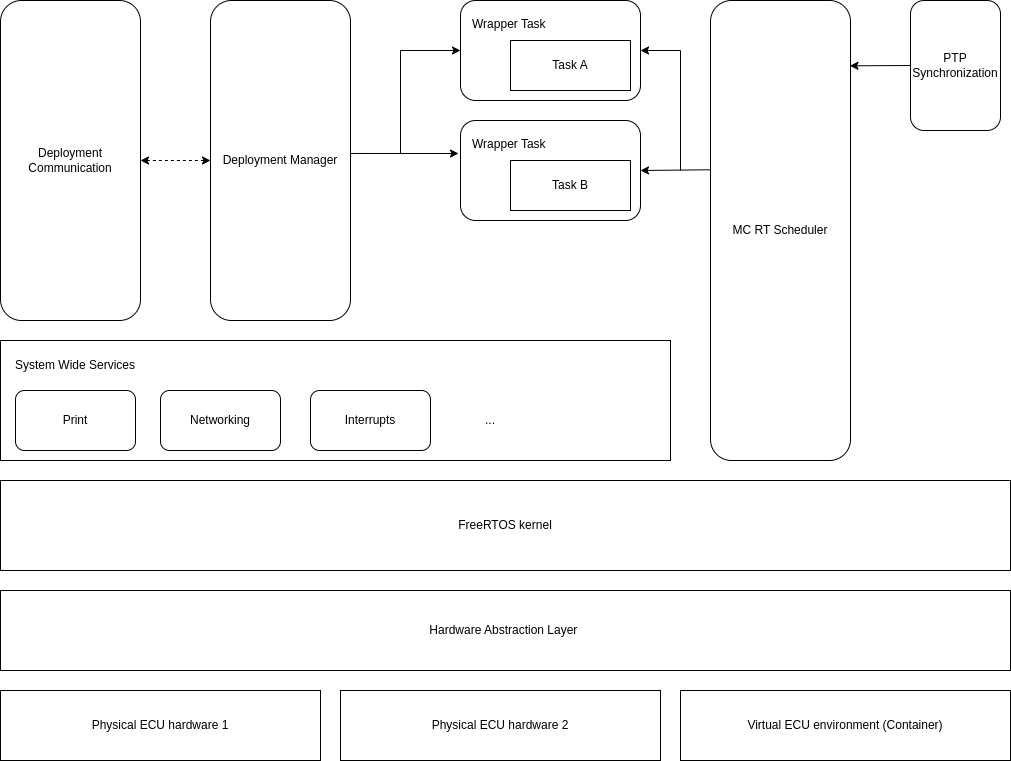
\includegraphics[width=\textwidth]{figures/os_arch_extended.png}}
	
	\caption{Axcan OS Architecture}
	\label{fig:os_arch}
\end{figure}

\begin{itemize}
	\item FreeRTOS Kernel and Hardware Abstraction Layer: These form the foundational runtime environment, providing deterministic task scheduling and hardware interfacing. Axcan OS builds on the FreeRTOS kernel to retain lightweight real-time execution.
	\item Task Deployment Communication Handler: Manages communication with the master node, including the reception of task binaries and instructions, and the transmission of runtime status information such as health metrics or migration readiness.
	\item Task Deployment Manager: Controls the full task lifecycle, including loading ELF applications into memory, instantiating them, starting or stopping execution, and handling checkpoint data for migration purposes. The deployment manager creates instances of the wrapper task that will contain the actual applications.
	\item Wrapper Task: Acts as a container for dynamically deployed user applications. It enables runtime execution of position-independent code by handling memory allocation, real-time constraints, and state checkpointing. It also provides user tasks with access to essential system functions through controlled interfaces.
	\item Extended Scheduler: Selects tasks for executing according to a policy. Configurable for implementing different simple real-time scheduling policies, not only non-criticality-aware ones like rate-monotonic, deadline-monotonic, and earliest-deadline-first, but also mixed-criticality aware approaches.
	\item System function services: Provides a minimal API for commonly needed services such as network communication or logging. These are abstracted through the microkernel and made available to user applications via the wrapper task, compensating for the lack of shared libraries in the FreeRTOS environment. 
	\item PTP Synchronization: Ensures global time alignment across nodes using the Precision Time Protocol (PTP), which is critical for maintaining timing guarantees and consistency during task migration.
\end{itemize}

Collectively, these components enable Axcan OS to serve as the runtime backbone for both physical and virtual ECU nodes within the breathable distributed system. The architecture ensures that all nodes — regardless of their underlying hardware or runtime context — can execute precompiled tasks under real-time constraints, coordinate with the master node, and participate in runtime task migration. Furthermore, Axcan OS is envisioned to work on both single-core and multi-core processors, as the multi-core approach treats each core as a sub-node , running copies of Axcan OS in every core in an asymmetric multi-processing (AMP) fashion, as shown in Fig. \ref{fig:multicore_example}, on the example of the ARM Cortex-A53, the processor present by the embedded devices used in the setup of this work. In such cases, core 0 typically acts as the master core and the rest of the cores as slave cores. The architecture of the OS for master and slave cores is almost identical, except for the deployment communication, as inter-core communication and internal task partitioning is also taken into account. The master node is also responsible for the management of system services, as most of them require a dedicated thread to own the resource to avoid conflicts, therefore offering an internal wrapper interface for system services on the other nodes. These differences are shown in Fig. \ref{fig:multicore_deployment_arch}, and the internal deployment of tasks is further explained in the next section.

\begin{figure}
	\centering
	\makebox[0.5\textwidth]{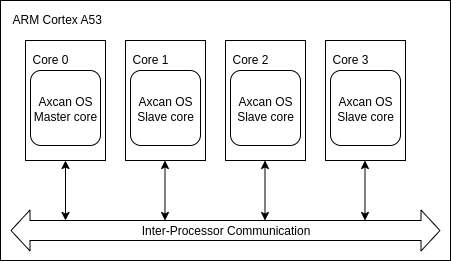
\includegraphics[width=0.5\textwidth]{figures/multicore_example.png}}
	
	\caption{Example of a multicore AMP system using Axcan OS}
	\label{fig:multicore_example}
\end{figure}

\begin{figure}
	\centering
	\makebox[0.75\textwidth]{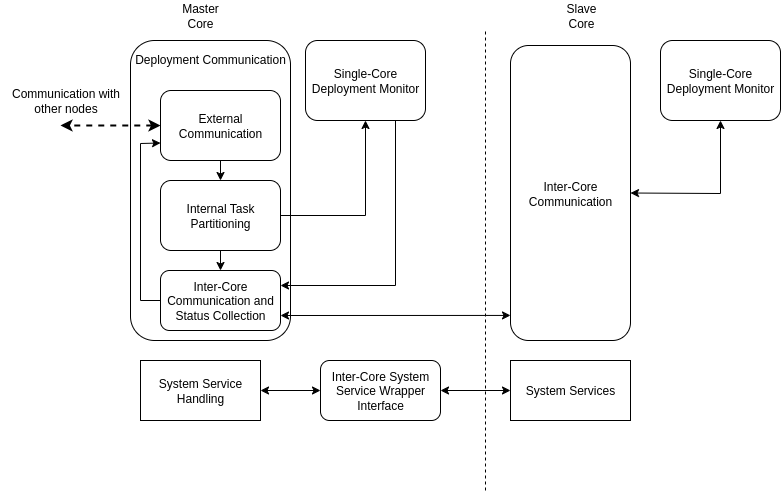
\includegraphics[width=0.75\textwidth]{figures/multicore_deployment_arch.png}}
	
	\caption{OS differences between master and slave cores}
	\label{fig:multicore_deployment_arch}
\end{figure}

The next sections explain into further detail how Axcan's components interact with each other to implement the features presented in the introduction of this chapter.

\section{Dynamic Task Deployment}
The vision of the breathable system requires ECUs to be able to execute different task loads depending on dynamic needs of the system, which change depending on different factors, such as external events and the availability of hardware resources. As one ECU represents a single node of the distributed system, and the execution of tasks is coordinated by the master node, Axcan includes a pair of tasks that act as an interface for deploying tasks remotely from the master node. First, the deployment communication thread is responsible for establishing a constant communication with the master node, exchanging status information about device health and current task load and status of each task. Also, this thread is responsible for receiving instructions from the master node regarding the execution of the assigned task set, which is then kept in a shared memory block and passed on to the deployment management thread. The deployment management thread is then responsible for handling the startup of the tasks and monitoring their status periodically. The startup includes first receiving the ELF and checkpoint files necessary for task execution, then allocating and initializing the memory required by the task, and finally creating the task thread and registering it in the mixed-criticality scheduler, which is then responsible for controlling when the CPU is given to the task. The monitoring sub-thread is then responsible for periodically checking whether the task is executing correctly, how many jobs have been executed, how many deadlines have been missed, etc. Furthermore, the monitoring is responsible also for pausing / stopping the tasks when told so by the master node, and for preparing and triggering the transfer of task files to another device when migration needs to occur.

\subsection{Multi-Core Deployment}
As shown in \ref{fig:multicore_deployment_arch}, multi-core nodes behave in a slightly different manner. First, the master core is the only one responsible for communicating with the master node for receiving deployed tasks. After receiving a task set, the master core distributes tasks internally via a greedy partitioning algorithm, aiming for a balanced task load among all cores. This algorithm considers an additional management load for the master core. A further extension of the partitioning is envisioned to handle mixed-criticality and avoiding the clash of multiple-criticalities on independent cores. After the partitioning process has been completed, the  master core sends internally the instructions to the slave cores and starts its own task load via the deployment monitor as described above. Slave cores then replace the communication task for an inter-core communication task, responsible for performing the intermediate communication with the master core, and then perform their normal workflow with the deployment monitor task. In both cases, the monitor task works in exactly the same manner as for single-core systems. The process for sending device and task status remains almost unchanged, only having the master-core collect the status of itself and the slave cores to send a general device status message to the master node in the distributed system. 


\section{Mixed-Criticality Scheduler}

The first step in achieving mixed criticality and respecting real-time behavior for the system applications is a scheduler that can achieve both goals. For this purpose, an extension of ESFREE (add reference), a project that implements a few dynamic and static real-time scheduling policies, including Earliest Deadline First (EDF), which for single core is ideally optimal (add references). This project is used as a base as the off-the-shelf FreeRTOS code only offers a priority-based scheduler, without any priority-assignment policies. In this work, the EDF policy is extended to cope with different levels of criticality by implementing the EDF with virtual deadlines for MC, as proposed in (add ref.).

**** Need to finalize implementing scheduling policies, then explain that into detail***

\section{Cross-Platform Task Loading}

To achieve the goal of executing the same application files on both physical and virtual ECU devices, the system integrates an ELF loader. This ELF loader, implemented to a great extent in collaboration with Yinbo Zhou in the scope of his master's thesis, enables the execution of multiple tasks, packed in the form of pre-compiled ELF files and with an additional data file. This approach tackles both challenges of allowing the dynamic loading of tasks and of stateful migration to the extent desired. In order for applications to be compatible with the task loader, they need to fulfill some requirements when compiled. The implemented loader is lightweight and meant to load the same application files on on multiple underlying hardware / software stacks, as shown in Fig. \ref{fig:multiplatform_tasks}, as long as an Axcan OS port runs on the target and the CPU architecture is the same as the target architecture for the compiled application, which in our case is always ARM Aarch64.


%\begin{figure}
%	\begin{minipage}{0.5\textwidth}
%	\centering
%	\makebox[0.9\textwidth]{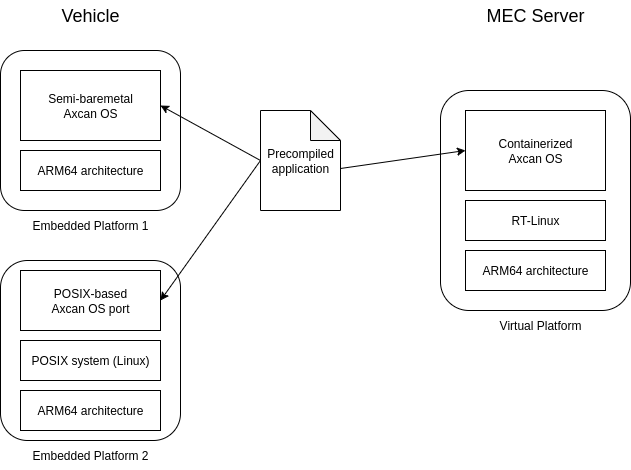
\includegraphics[width=0.9\textwidth]{figures/multiplatform_task_compatibility.png}}
%	
%	\caption{Cross-Platform Task Compatibility}
%	\label{fig:multiplatform_tasks}
%	\end{minipage}
%	\begin{minipage}{0.5\textwidth}
%	\centering
%	\makebox[0.85\textwidth]{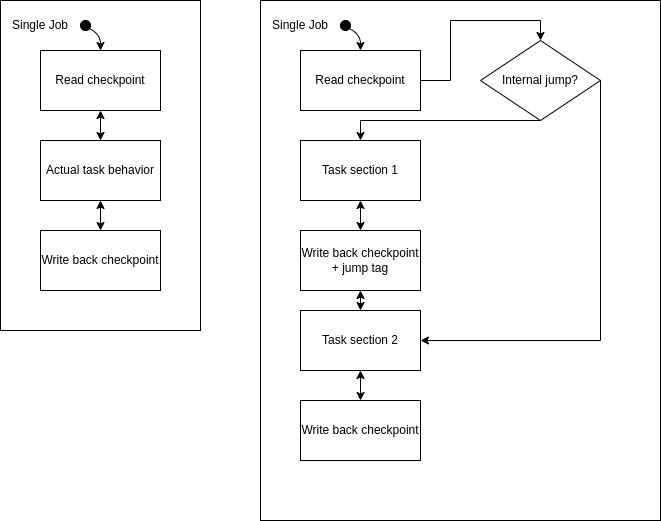
\includegraphics[width=0.85\textwidth]{figures/Task_arch.png}}
%	
%	\caption{User Application Flow}
%	\label{fig:user_app_design}
%	\end{minipage}
%\end{figure}

\begin{figure}
	\centering
	\makebox[0.6\textwidth]{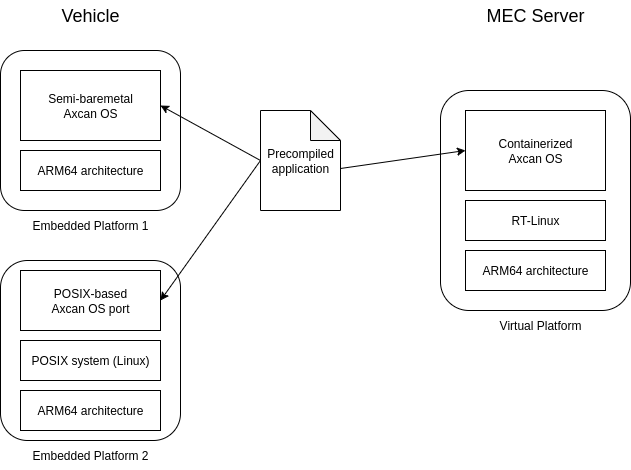
\includegraphics[width=0.6\textwidth]{figures/multiplatform_task_compatibility.png}}
	
	\caption{Cross-Platform Task Compatibility}
	\label{fig:multiplatform_tasks}
\end{figure}

\begin{figure}
	\centering
	\makebox[0.6\textwidth]{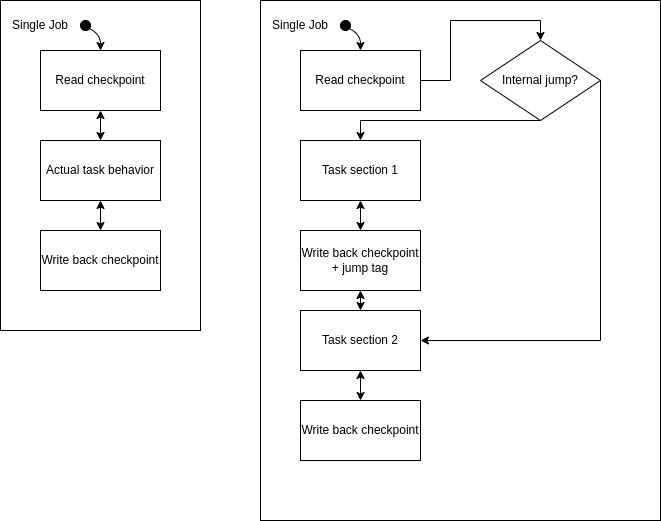
\includegraphics[width=0.6\textwidth]{figures/Task_arch.png}}
	
	\caption{User Application Flow}
	\label{fig:user_app_design}
\end{figure}

\subsection{Hardware Abstraction Layer}
In order to achieve full compatibility across different platforms, an abstraction layer is added under Axcan OS. This layer ensures applications can run on any target platform independently of the hardware and software stack, apart from the architecture. The use of FreeRTOS kernel official ports already allows an abstraction layer in the form of FreeRTOS features, but due to the lightweight implementation of FreeRTOS, some features remain specific to the underlying platform, which is also undesired when aiming to load the same ELF file on different platforms. To achieve this, two core features are included as part of the extended kernel of Axcan OS. First, most of the system calls are encapsulated in wrappers, e.g.: the console output, network features, memory management, access to other peripherals, which are then offered via a standard signature that internally calls the proper underlying code. Second, the ELF loader, apart from processing the ELF and performing the needed relocations, needs to allocate memory for ELF execution, which should be aligned properly for the respective platform. This means that for hardware specific ports of FreeRTOS, which run on a bare metal system, memory can be allocated without any underlying considerations, but also requiring some memory management handling if no memory management unit (MMU) is available on the port. On the other hand, ports based on the POSIX port of FreeRTOS (e.g. the container approach running on a Linux server or even versions running as processes on top of UNIX based OSs) should take into consideration that the underlying OS is responsible for memory management, often not allowing standard \textit{malloc} calls to hold executable code. This specific case means that alternative memory allocation functions, such as \textit{mmap}, which are more flexible but require a more explicit memory handling in code, should be used. 


\subsection{User Application Requirements}
User applications need to meet two requirements to be compatible with Axcan OS. First, they need to be compiled with the right flags, particularly by enabling position independent execution (PIE) and to avoid integration of standard C libraries and system startup functions (they should use newlib to allow for applications to be encapsulated without dynamic library linking). Second, they should use the Axcan OS header and library files, which will provide access to basic system functions and core features, such as the checkpoint mechanism, the resource table for checkpoint variable handling and the proper entrypoint handling. System services are offered through global function pointers. All those elements are initialized by the operating system and passed to user applications through a data structure in shared memory.

Furthermore, by design user applications are periodic and must define and keep track of the state-relevant variables for their further execution, meaning that the main function acts as a single job execution, and any execution context needed for a job must be loaded at the beginning of the main and stored back at the end. This represents the minimal checkpoint version where state is only resumed from the beginning of a job. Further checkpoints can also be added in the middle of the code in the form of internal jumps that need to be executed at the start of the main function, allowing the job to resume also from internal points. These two cases are shown in Fig. \ref{fig:user_app_design}.

\section{Summary}

This chapter introduced Axcan OS, the lightweight real-time operating system designed to serve as the execution environment for both physical and virtual nodes in the proposed breathable distributed system. Building upon the FreeRTOS microkernel, Axcan OS was extended with custom components to meet the core functional requirements for allowing single nodes to be integrated in the overall distributed real-time system, namely dynamic deployment of real-time tasks, task migration and execution across heterogeneous platforms and handling of tasks with different criticalities.

The modular architecture of Axcan OS, along with its internal mechanisms, as explained in this chapter, implement the backbone for the behavior of the ECU nodes, making it possible for them to work as parts of a single system. This integration of different nodes is the base for the features explained in the next chapters, such as the task migration strategies, the real-time considerations in the distributed system and the task allocation to specific nodes.

It is relevant to note that at the moment of writing, Axcan OS is implemented as a proof-of-concept framework. Further work is needed to provide a wider set of system services to user applications, and possibly to provide more efficient communication mechanisms among nodes in the distributed system.

